\documentclass{beamer}
\usepackage{graphicx}

\title{Committee meeting for Connor Burbridge}
\subtitle{Committee members: Dave Schneider, Tony Kusalik, Matthew Links, Leon Kochian}
\author{Connor Burbridge}
\date{\today}

\begin{document}
\begin{frame}
  \titlepage
\end{frame}

\begin{frame}
  \frametitle{Project Proposal Outline}
  \begin{itemize}
  \item Background
  \item Research Problem
  \item Current Progress
  \item Timeline
  \item Deliverables
  \end{itemize}
\end{frame}

\begin{frame}
  \frametitle{Background: \textit{Trichoderma}}
  What is \textit{Trichoderma}?
  \begin{itemize}
  \item \textit{Trichoderma} is an opportunistic symbiotic fungi, which
    can colonize the roots of plants
  \item \textit{Trichoderma} strains have been shown to provide
    several benefits to the host plant it colonizes, those generally
    being:
    \begin{itemize}
      \item Increased resistance to abiotic and biotic stressors
      \item Facilitating nutrient uptake
      \item Increased germination rates
    \end{itemize}
  \item These benefits have resulted in \textit{Trichoderma} being
    used in manufacturing processes for antibiotics and other materials
  \end{itemize}
\end{frame}

\begin{frame}
  \frametitle{Background: Previous GIFS Work}
  Two strains have been sequenced in previous work within GIFS:
  \begin{itemize}
  \item These strains have been named DC1 and Tsth20
  \item Strains from the prairie regions of Canada, including Alberta
    and Saskatchewan
  \item How exactly do these processes work? Which genes are included
    in these processes?
  \item To answer these questions, both strains were sequenced with
    Illumina and Nanopore technologies
  \end{itemize}
\end{frame}

\begin{frame}
  \frametitle{Research Problem} These sequenced strains offer an
  opportunity to assemble and annotate them:
  \begin{itemize}
  \item Genome assembly is 'relatively' straight-forward
  \item \textbf{However, the choice of a tool for gene finding or
    annotation is uncertain}
  \item There has been relatively little comparative analysis for gene
    finding tools in fungi, and even fewer for \textit{Trichoderma}
  \item \textbf{This raises questions. How do different gene finding
    tools perform in fungi and \textit{Trichoderma} in particular?}
  \end{itemize}
\end{frame}

\begin{frame}
  \frametitle{Project Goal} \textbf{This project aims to evaluate
    several different gene finding tools in the context of
    \textit{Trichoderma} genomes}
  \begin{itemize}
    \item Gene finding tools currently selected are GeneMark-ES,
      GenomeThreader, and Braker2
    \item These tools include a mix of \textit{ab initio},
      evidence-based and hybrid gene finding methods
    \item This list is not final and may include more tools if
      desired or necessary
  \end{itemize}
\end{frame}

\begin{frame}
  \frametitle{Evaluation of Gene Finding Tools} A methodology for
  evaluating and comparing the selected tools needs to be
  developed. Metrics for comparison will include:
  \begin{itemize}
  \item Efficiency of selected gene finding tools
  \item Requirements of selected gene finding tools and ease of
    installation
  \item Comparison and validation of called genes with existing RNASeq data if
    available
  \item Identification of small RNAs and genes in repetitive and
    AT-rich regions
  \item Distribution of lengths of called genes (particularly in the
    case of \textit{ab initio} gene finders)
  \end{itemize}
\end{frame}

\begin{frame}
  \frametitle{Current Progress}
  Preliminary assemblies for both DC1 and Tsth20 are ready
  \begin{itemize}
  \item Two assemblies for each strain using both SPAdes and MaSuRCA
  \item Both assemblers use a hybrid assembly approach
  \end{itemize}
\end{frame}

\begin{frame}
  \frametitle{Assembly Metrics}
  SPAdes
  \begin{center}
  \resizebox{\textwidth}{!}{
    \begin{tabular}{|c|c|c|c|c|c|c|}
      \hline
      Strain & Total Contigs & Total Length & Largest Contig & GC\% & N50 & L50 \\ \hline
      Tsth20 & 611 & 41.88 Mb & 2.44 Mb & 47.28 & 1.17 Mb & 14 \\ \hline
      DC1 & 181 & 38.60 Mb & 1.85 Mb & 47.95 & 807.44 Kb & 17 \\ \hline 
    \end{tabular}
    }
    \label{table1} \vspace{0.5cm}
  \end{center}
  MaSuRCA
  \begin{center}
  \resizebox{\textwidth}{!}{
    \begin{tabular}{|c|c|c|c|c|c|c|}
      \hline
      Strain & Total Contigs & Total Length & Largest Contig & GC\% & N50 & L50 \\ \hline
      Tsth20 & 8 & 41.52 Mb & 9.97 Mb & 47.36 & 4.96 Mb & 3 \\ \hline
      DC1 & 13 & 38.60 Mb & 7.36 Mb & 47.96 & 4.06 Mb & 4 \\ \hline 
    \end{tabular}
    }
  \label{table1} \vspace{0.5cm}
  \end{center}
\end{frame}

\begin{frame}
  \frametitle{Existing Progress Cont.}
  AT-rich regions of assembled DC1 genomes (SPAdes left, MaSuRCA right):
  \begin{center}
    \includegraphics[width=0.45\textwidth]{/Users/cbe453/Desktop/masters/GC-content/dc1-spades-gccontent.pdf}
    \includegraphics[width=0.45\textwidth]{/Users/cbe453/Desktop/masters/GC-content/dc1-masurca-gccontent.pdf}
  \end{center}
\end{frame}

\begin{frame}
  \frametitle{Existing Progress Cont.}
  AT-rich regions of assembled Tsth20 genomes (SPAdes left, MaSuRCA right):
  \begin{center}
    \includegraphics[width=0.45\textwidth]{/Users/cbe453/Desktop/masters/GC-content/tsth20-spades-gccontent.pdf}
    \includegraphics[width=0.45\textwidth]{/Users/cbe453/Desktop/masters/GC-content/tsth20-masurca-gccontent.pdf}
  \end{center}
\end{frame}

\begin{frame}
  \frametitle{Existing Progress Cont.}
  AT-rich regions in GenBank assembly of \textit{Trichoderma reesei}:
  \begin{center}
    \includegraphics[width=0.45\textwidth]{/Users/cbe453/Desktop/masters/GC-content/t-reesei-gccontent.pdf}
  \end{center}
\end{frame}

\begin{frame}
  \frametitle{Existing Progress Cont.}
  Mauve Alignments for DC1 MaSuRCA Assembly:
  \begin{center}
    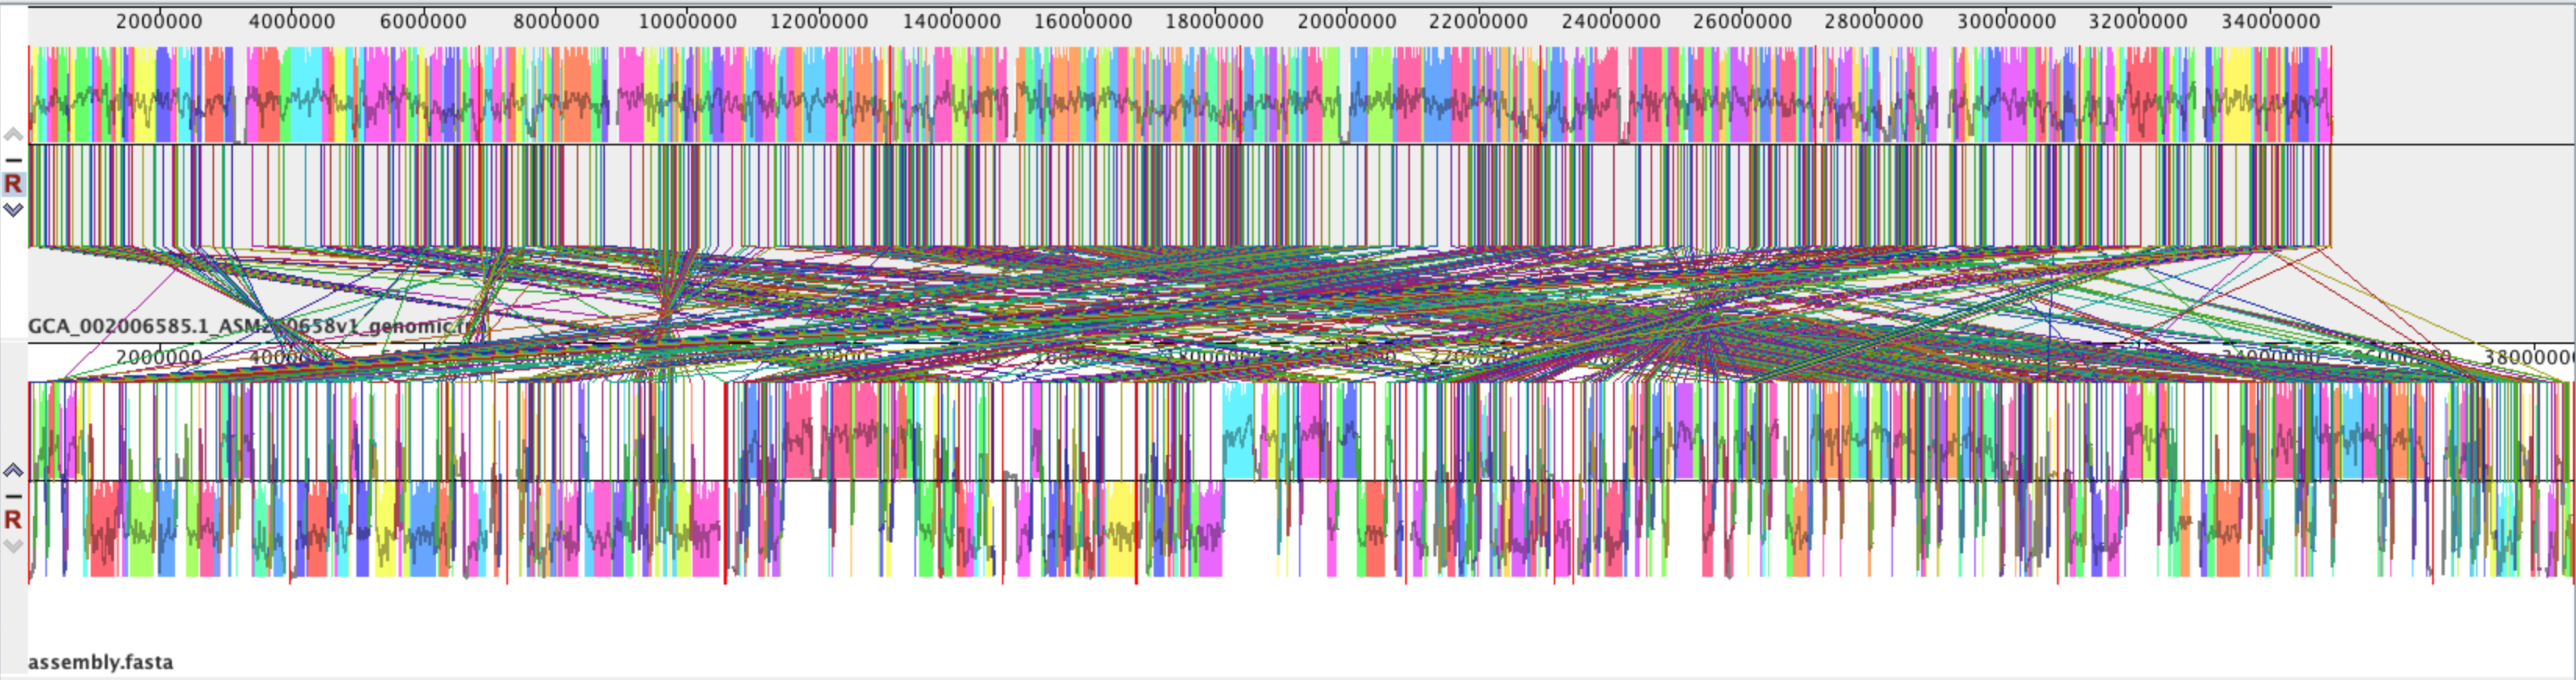
\includegraphics[width=\textwidth]{/Users/cbe453/Desktop/masters/committee-meetings/mauve-images/dc1-masurca-treesei.png}
  \end{center}
\end{frame}

\begin{frame}
  \frametitle{Existing Progress Cont.}
  Mauve Alignments for Tsth20 MaSuRCA Assembly:
  \begin{center}
    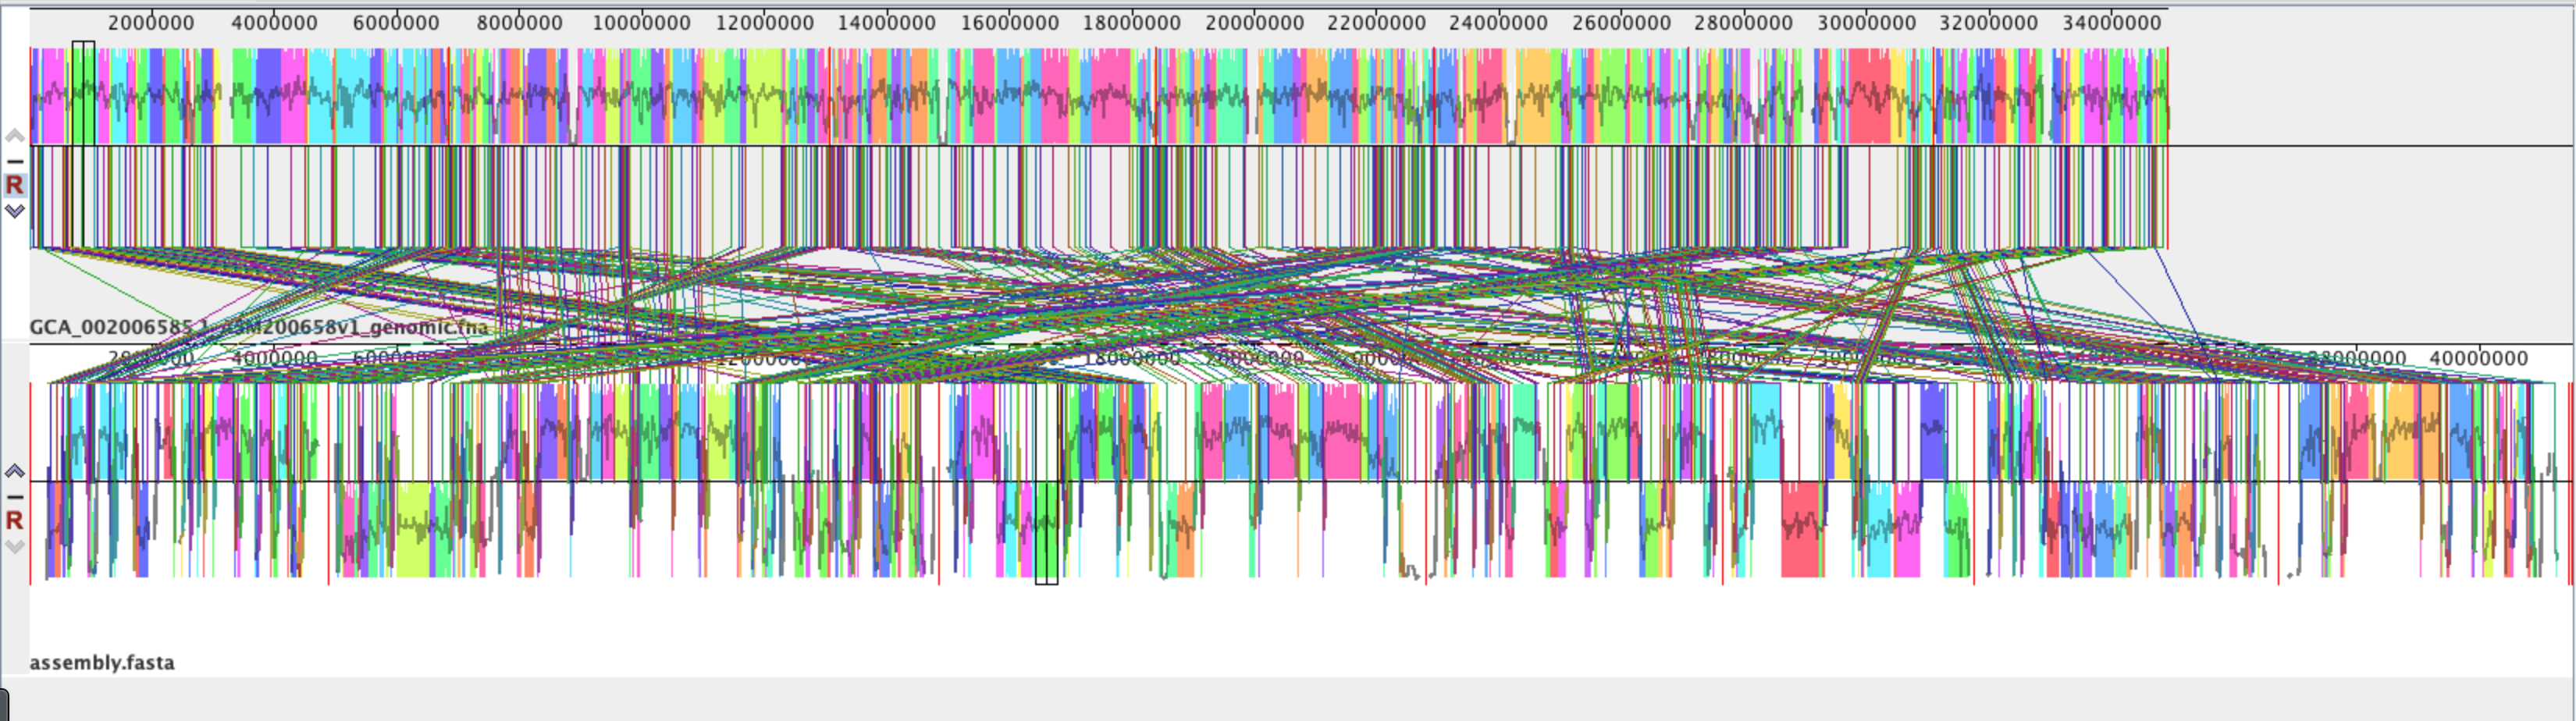
\includegraphics[width=\textwidth]{/Users/cbe453/Desktop/masters/committee-meetings/mauve-images/tsth20-masurca-treesei.png}
  \end{center}
\end{frame}

\begin{frame}
  \frametitle{Next Steps}
  \begin{itemize}
  \item Finish assemblies of DC1 and Tsth20
  \item Identify repetititve regions of selected assemblies
  \item Identify non-coding RNAs in selected assemblies
  \item Apply gene finders to selected assemblies and evaluate
  \end{itemize}
\end{frame}

\begin{frame}
  \frametitle{Deliverables}
  \begin{itemize}
  \item Assemblies of both Tsth20 and DC1
  \item Lists of potential genes for each \textit{Trichoderma}
    assembly considered
  \item A consensus or core gene set for genes called by all gene
    finders
  \item Repetitive regions identified in all \textit{Trichoderma}
    genomes considered
  \item Potential true positives supported by RNAseq evidence and
    existing annotations
  \item Final comparative tables including the evaluation metrics
    described previously
  \end{itemize}
\end{frame}

\begin{frame}
  \frametitle{Timeline}
  \begin{itemize}
  \item Finishing assemblies of DC1 and Tsth20 assemblies (2 weeks)
  \item Collection of existing genome assemblies (1 week)
  \item Application of gene finding tools to selected genomes (1-2
    months)
  \item Downstream analysis of gene finding results (1-2 months)
  \end{itemize}
\end{frame}

\begin{frame}
  \begin{center}
    Questions and/or comments
  \end{center}
\end{frame}

\end{document}
